
% ------------------------------------------------
% --- TRACK FUSION EVALUATION --------------------
% ------------------------------------------------

\chapter{Track Fusion: Design and Evaluation} \label{cha:track-fusion-evaluation}

Track fusion is a crucial component of a \abbrDTT system. In this chapter we will discuss how the design and evaluation of the track fusion component as part of a \abbrDTT system in a single-target configuration. One such configuration is illustrated in Figure~\ref{fig:dstt:sst-scenario}, where multiple agents measure and track a common target, and communicate the local tracks with the other agents for track fusion. In the single-target context, the \abbrDTT system reduces to state estimation, track fusion, and communication management. The choice of track fusion method is a compromise between \emph{tracking performance}, which is related to the computed covariance of the track, and \emph{uncertainty assessment}, which is related to conservativeness. It should be stressed that there is no track fusion method that is best in general problems. The most suitable track fusion for a certain problem essentially depends solely on the user needs. %For instance, it might be beneficial to sacrifice conservativeness for better tracking performance.

This chapter starts by describing state estimation and track fusion. Several important evaluation measures are then described. We finally discuss how to design and evaluate a track fusion component.

\begin{figure}[b]
	\centering
	\begin{tikzpicture}[scale=.25]
		
% AGENTS
\def\ra{0.75}




% --- FIGURE ---
\BFS

\drawtargettrajectory [path fading=east] plot [smooth, tension=1] coordinates {(0,0) (7,5) (15,1) (24,3) (30,4)};
\node at (0,0) {\mycircle{black}};


% AGENT 1
\def\xa{(-8,3)}
\draw [rotate around={-20:\xa}] \sensoropt{clra} \xa -- (-3,5) to [out=-60,in=60] (-3,1) -- cycle;	
\drawcomarrow[->,rotate around={11:\xa}] \xa -- (-4,3);
\drawagent{clra} \xa circle [radius = \ra];


% AGENT 2
\def\xa{(15,8)}
\draw [rotate around={-140:\xa}] \sensoropt{clrb} \xa -- (20,10) to [out=-60,in=60] (20,6) -- cycle;
\drawcomarrow[->,rotate around={11:\xa}] \xa -- (11,8);
\drawcomarrow[->,rotate around={-35:\xa}] \xa -- (19,8);
\drawagent{clrb} \xa circle [radius = \ra];


% AGENT 3
\def\xa{(27,0)}
\draw [rotate around={180:\xa}] \sensoropt{clrc} \xa -- (32,2) to [out=-60,in=60] (32,-2) -- cycle;	
\drawcomarrow[->,rotate around={-35:\xa}] \xa -- (23,0);
\drawagent{clrc} \xa circle [radius = \ra];


\EFS
	\end{tikzpicture}	
	\caption{A single-target tracking scenario. Multiple agents (colored circles) track a dynamic target (black circle) using sensors (colored cones) and internal processing units. The agents exchange local track estimates over a datalink (dotted arrows) for track fusion. } 
	\label{fig:dstt:sst-scenario}
\end{figure}




% --- MODELING ---
\section{A Decentralized Single-Target Tracking System}

In the single-target tracking case, the measurement-to-track association and track-to-track association are often trivial or already solved and therefore can be disregarded. This case is assumed here. Hence, the \abbrDTT system comprises state estimation, track fusion, and communication management. A decentralized single-target tracking system is illustrated in Figure~\ref{fig:intro:dstt-system}.

\begin{figure}[t]
	\centering
	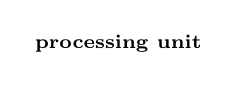
\begin{tikzpicture}[scale=.9]
		
% --- FIGURE ---
\begin{scriptsize}

%\draw [white,opacity=.0] (0,-1) rectangle (17,0);

\drawprocessingunitbox{clra!40!} (2.75,-1.75) rectangle (9.75,2);
\node [below,font=\bfseries] at (6.25,2) {processing unit};

% STATE EST
\drawsensorbox (0,0) rectangle (2,1) node [pos=.5,font=\bfseries,color=white] {sensors};
\drawsystemarrow (2,0.5) -- (3,0.5);
\drawsystembox (3,0) rectangle (5.5,1) node [pos=.5,font=\bfseries,align=center] {state \\ estimation};
\drawsystemarrow (4.25,0) -- (4.25,-0.5);

% FUSION
\drawsensorbox (0,-0.5) rectangle (2,-1.5) node [pos=.5,font=\bfseries,align=center,color=white] {datalink};
\drawsystemarrow (2,-1) -- (3,-1);
\drawsystembox (3,-0.5) rectangle (5.5,-1.5) node [pos=.5,font=\bfseries,align=center] {track \\ fusion};

% COM
\drawsystemarrow (5.5,-1) -- (6.5,-1);
%\drawsystemarrow [densely dashed] (10.75,-1) -- (10.75,1.25) -- (5,1.25) -- (5,1);
%\draw [black,fill=black] (10.75,-1) circle [radius=0.05];
\drawsystembox (6.5,-0.5) rectangle (9.5,-1.5) node [pos=.5,font=\bfseries,align=center] {communication \\ management};
\drawsystemarrow (9.5,-1) -- (10.5,-1) node [near start,above right,align=center,font=\it] {exchanged \\ track};

\end{scriptsize}
	\end{tikzpicture}
	\caption{A decentralized single-target tracking system. }
	\label{fig:intro:dstt-system}
\end{figure}

The focus here is the design and evaluation of track fusion, but we need to also briefly discuss state estimation as this is an important part as well. However, to be able to analyze track fusion we want the state estimation to be well-tuned in the case of no fusion. If the state estimation is not sufficiently tuned, then it will be difficult to evaluate the track fusion as it becomes very hard to see if it the assessed performance and conservativeness is due to the state estimation or the track fusion. The communication management is discussed in the subsequent chapter.




% STATE ESTIMATION
\subsection{State Estimation}

Let $x_k\in\realsnx$, where $\nx$ is the dimensionality, be the target state at time $k$. In the thesis there is an explicit differentiation between a random variable and a realization thereof. Random variables are bold face, \eg, $\bfa$, and realizations are normal face, \eg, $a$. This notation is kept here for consistency. The expectation value of $\bfa$ is denoted $\EV(\bfa)$. The covariance of $\bfa$ is denoted $\cov(\bfa)$ and $\cov(\bfa,\bfb)$ is the cross-covariance between $\bfa$ and $\bfb$.

A \emph{state-space model} (\abbrSSM) is used to describe the state and measurements of the target. The \abbrSSM comprises a \emph{process model} for the target dynamics and a \emph{measurement model} that relates measurements to the target state. A family of discrete time SSMs is given by
\begin{subequations} \label{eq:model:ssm}
\begin{align}
x_{k+1} &= F_kx_k + w_k, & \bfw_k &\sim\calN(0,Q_k), \\
z_k &= h(x_k) + e_k, & \bfe_k &\sim\calN(0,C_k),
\end{align}
\end{subequations}
where $F_k$ is the state transition model, $Q_k$ is the covariance of the process noise $\bfw_k$, $z_k$ is a measurement vector, $h$ is a nonlinear measurement function, and $C_k$ is the covariance of the measurement noise $\bfe_k$. It is assumed that $\cov(\tbfx_{k|l},\bfw_k)=0$ for all $k\geq l$, where $\tbfx_{k|l}=\hbfx_{k|l}-x_k$. Moreover, it is assumed that $\cov(\bfw_k,\bfe_l)=0$ for all $k,l$. Subscript $k|l$ denotes filtered quantities evaluated at time $k$ using measurements up to and including time $l$.

The \abbrSSM in \eqref{eq:model:ssm} is assumed throughout the thesis. The process model is linear, but the measurement model in general involves a nonlinear function. The \abbrEKF \cite{Jazwinski1970} in Algorithm~\ref{alg:ekf} is used to recursively compute a state estimate of $x_k$ using a time update and a measurement update in each filter recursion. If $h(x_k)=H_kx_k$, then the \abbrEKF in Algorithm~\ref{alg:ekf} reduced to the linear Kalman filter (\abbrKF, \cite{Kalman1960}). In this scope $(\xhat\kk,P\kk)$ is referred to as a \emph{track}. See \cite{Forsling2023Phd} for more information about relevant process and measurement models.

\begin{algorithm}[tb]
	\caption{Extended Kalman Filter}
	\label{alg:ekf}
	\begin{small}
	\begin{algorithmic}[0]
		\Input State-space model \eqref{eq:model:ssm}, initial values $\xhat_{0|0}=\xhat_0$ and $P_{0|0}=P_0$
		\State Time update:
		\begin{align}
			\xhat\kpk &= F_k\xhat\kk, & P\kpk &= F_kP\kk F_k\trnsp + Q_k.
		\end{align}
		\State Measurement update:
		\begin{align}
			\xhat\kk &= \xhat\kkm + K_k\left(z_k-h(\xhat\kkm)\right), & P\kk &= (I-K_kH_k)P\kkm,
		\end{align}		
		\State where $K_k = P\kkm H_k\trnsp(H_kP\kkm H_k\trnsp+C_k)\inv$ and $H_k = \left.\frac{\partial h(x')}{\partial x'}\right\vert_{x'=\xhat\kkm}$.
		\Output $(\xhat_{k|k},P_{k|k})$
	\end{algorithmic}
	\end{small}
\end{algorithm}


% FILTER TUNING
\subsubsection{Filter Tuning}

All local filters need to be tuned for their particular applications. For well-designed sensors, this essentially boils down to designing the process noise covariance $Q_k$. A systematic approach to filter tuning is described in \cite{Bar-Shalom2001}. The authors of \cite{Chen2018Fusion} propose a methodology for auto-tuning of filters. In this scope, we just assume that the filter has already been tuned. 




% TRACK FUSION
\subsection{Track Fusion}

In \abbrDTT, tracks and covariances are exchanged between agents. The performance of the \emph{track fusion} depends on the fusion rule used to combine tracks. In essence, this fusion rule is an estimator. The following notation is used when describing track fusion:
\begin{itemize}
	\item The local tracks to be fused are represented by $(y_1,R_1),\dots,(y_N,R_N)$, where $(y_i,R_i)$ is the local track in Agent~$i$ and $N$ is the number of agents. For instance, assume Agent~1 and Agent~2 compute local tracks, \eg, using EKFs, and that these local tracks are fused in Agent~2. Then it is said that Agent~1 transmits $(y_1,R_1)$ to Agent~2 who fuses $(y_1,R_1)$ with its local track $(y_2,R_2)$.
	\item The estimate computed in the track fusion is denoted $(\xhat,P)$.
\end{itemize}
Track fusion is an instantaneous operation, where two or more tracks evaluated at the same time are merged. This means, in contrast to state estimation, that time indices in general can be disregarded when describing track fusion. %Nevertheless, for clarity, it is sometimes needed to use time indices for $(y_i,R_i)$. In such a case, the local track is denoted $(y_{i,k},R_{i,k})$, and the fused result is denoted $(\xhat_{i,k},P_{i,k})$.

An important special case in the thesis is the fusion of $\nagent=2$ local estimates given as
\begin{subequations} \label{eq:model:two-estimates}
\begin{align}
	y_1 &= x + v_1, & R_1=\cov(\bfv_1), \\
	y_2 &= H_2x + v_2, & R_2=\cov(\bfv_2),
\end{align}	
\end{subequations}
where $x$ is the target state (with time index omitted). The cross-covariance between $\bfy_1$ and $\bfy_2$ is denoted $R_{12}=\cov(\bfy_1,\bfy_2)$. Note, in many fusion problems $H_2=I$, where $I$ is the identity matrix.


% CONSERVATIVE EST
\subsubsection{Conservative Estimation}

An estimator, or fusion method, that computes $(\xhat,P)$, where $\xhat$ is an estimate of $x$ and $P$ the computed covariance of $\xhat$, is \emph{conservative} \textiff 
\begin{equation}
	P - \EV(\tbfx\tbfx\trnsp) \succeq 0,
	\label{eq:def:conservative-est}
\end{equation}
where $\tbfx=\hbfx-x$ and $A-B\succeq 0$ means that the difference $A-B$ is positive semidefinite. The notion of conservative has been introduced in distributed/decentralized estimation due to the difficulty of correct uncertainty assessment. This difficulty typically arises because the cross-covariance, \eg, $R_{12}$, is unknown. This is also what we mean when we say that the ''correlations are unknown''. If nonzero $R_{12}$ is ignored, then \eqref{eq:def:conservative-est} typically does not hold and the true covariance $\EV(\tbfx\tbfx\trnsp)$ is underestimated.

Figure~\ref{fig:example:conservative-nonconservative-estimate} illustrates the ellipses\footnote{The ellipsoid of an $n\times n$ symmetric positive definite matrix $S$ is given by the set of points $\calE(S)=\{a\in\realsn\,|\, a\trnsp S\inv a\leq 1\}$.} of the covariances of a conservative estimate $(\xhat,P)$ and a non-conservative estimate $(\xhat^n,P^n)$.

\begin{figure}[tb]
	\centering
	\begin{tikzpicture}[scale=.4]
		
\def\drawtrue{\draw[ultra thick,dashed,black]}
\def\drawcons{\draw[ultra thick,mydarkgreen]}
\def\drawnon{\draw[ultra thick,myred]}

\def\Ptrue{(0,0)ellipse[x radius = 4, y radius = 1.5, rotate = 20];}

\def\xleg{-5}
\def\yleg{4.5}
\def\lleg{1}
\def\sleg{12}





% --- FIGURE ---
\BFS


% LEFT
\drawtrue\Ptrue
\drawcons (0,0) ellipse [x radius = 5, y radius = 2, rotate = 25];
\node at (0,0) {$P\succeq\EV(\tbfx\tbfx\trnsp)$};


% RIGHT
\begin{scope}[xshift=16cm]
	
\drawtrue\Ptrue
\drawnon (0,0) ellipse [x radius = 5, y radius = 2, rotate = -25];	
\node at (0,0) {$P^n\not\succeq\EV(\tbfx\tbfx\trnsp)$};
	
\end{scope}


% LEGEND
\drawcons({\xleg},\yleg)--({\xleg+\lleg},\yleg) node [right,black] {$P$};
\drawtrue ({\xleg+\sleg},\yleg)--({\xleg+\lleg+\sleg},\yleg) node [right,black] {$\EV(\tbfx\tbfx\trnsp)$};
\drawnon ({\xleg+2*\sleg},\yleg)--({\xleg+\lleg+2*\sleg},\yleg) node [right,black] {$P^n$};




\EFS

	\end{tikzpicture}
	\caption{A conservative estimate and a non-conservative estimate.}
	\label{fig:example:conservative-nonconservative-estimate}
\end{figure}


% TF METHODS
\subsubsection{Track Fusion Methods}

Three relevant track fusion methods are now stated. These methods will be used to illustrate the track fusion design and evaluation. There are many other methods that might be consider, see the thesis \cite{Forsling2023Phd} for additional track fusion methods. The thesis also describe a general optimization based framework for track fusion. However, for the sake of simplicity, this framework has been excluded here.

The measurement update of a Kalman filter can be used to fuse two (or more) tracks. This type of fusion is henceforth denoted the \emph{Kalman fuser} (\abbrKF), and is defined in Algorithm~\ref{alg:kf} for the model in \eqref{eq:model:two-estimates}. In fact, if $R_{12}=0$, then the \abbrKF is optimal. If \abbrKF is used when $R_{12}\neq 0$, then the fused result is not conservative\footnote{The case when \abbrKF is used despite $R_{12}\neq 0$ is often referred to as \emph{\naive fusion} or \emph{\naive \abbrKF}.}. However, it is still useful to include \abbrKF in the track fusion design---not at least as a baseline method. In particular, \abbrKF is often the preferred choice when some decorrelation step has been implemented\footnote{Decorrelation here refers to the process of subtracting an estimate from another such that the new estimate is (approximately) uncorrelated with the estimate(s) to be fused with.}.

\begin{algorithm}[tb]
	\caption{Kalman Fuser}
	\label{alg:kf}
	\begin{small}
	\begin{algorithmic}[0]
		\Input $(y_1,R_1)$, $(y_2,R_2)$, and $H_2$
		\State The estimates are fused according to:
		\begin{align} 
			\xhat &= P(R_1\inv y_1 + H_2\trnsp R_2\inv y_2), & P &= (R_1\inv + H_2\trnsp R_2\inv H_2 )\inv.
			\label{eq:method:kalman-fuser-2est}
		\end{align}
		\Output $(\xhat,P)$
	\end{algorithmic}
	\end{small}
\end{algorithm}



\emph{Covariance intersection} (\abbrCI, \cite{Julier1997ACC}) is one of the most popular methods for fusing estimates under unknown correlations. \abbrCI is provided in Algorithm~\ref{alg:ci} for the fusion of two estimates defined as in \eqref{eq:model:two-estimates}. It has been shown that \abbrCI always provide a conservative estimate given that the estimates to be fused are conservative.

\begin{algorithm}[tb]
	\caption{Covariance Intersection}
	\label{alg:ci}
	\begin{small}
	\begin{algorithmic}[0]
		\Input $(y_1,R_1)$, $(y_2,R_2)$, and $H_2$
		\State The estimates are fused according to:
		\begin{align} 
			\xhat &= P(\omega R_1\inv y_1 + (1-\omega)H_2\trnsp R_2\inv y_2 ), & P &= (\omega R_1\inv + (1-\omega)H_2\trnsp R_2\inv H_2)\inv,
			\label{eq:method:ci-2est}
		\end{align}
		with $\omega$ given by
		\begin{equation}
			\begin{aligned}
				& \underset{\omega}{\minimize}& & J(P),
			\end{aligned}
		\end{equation}
		for a matrix increasing function $J(P)$, \eg, $J(P)=\trace(P)$.
		\Output $(\xhat,P)$
	\end{algorithmic}
	\end{small}
\end{algorithm}



The \emph{largest ellipsoid} (\abbrLE, \cite{Benaskeur2002IECON}) method\footnote{The \abbrLE method has also been named \emph{safe fusion} \cite{Gustafsson2018} and \emph{ellipsoidal intersection} \cite{Sijs2010ACC}.} is a less conservative alternative to \abbrCI. A generalization of the \abbrLE method is provided in Algorithm~\ref{alg:le}.

\begin{algorithm}[tb]
	\caption{The Largest Ellipsoid Method}
	\label{alg:le}
	\begin{small}
	\begin{algorithmic}[0]
		\Input $(y_1,R_1)$, $(y_2,R_2)$, and $H_2$
		\State The estimates are fused according to:
		\begin{enumerate}
			\item Transform to the information domain
			\begin{align*}
				\iota_1 &= R_1\inv y_1, & \calI_1 &= R_1\inv, &
				\iota_2 &= H_2\trnsp R_2\inv y_2, & \calI_2 &= H_2\trnsp R_2\inv H_2.
			\end{align*}
			\item Factorize $\calI_1=U_1\Sigma_1U_1\trnsp$ and let $T_1=\Sigma_1\invsqrt U_1\trnsp$. Factorize $T_1\calI_2T_1\trnsp=U_2\Sigma_2U_2\trnsp$ and let $T_2=U_2\trnsp$. Transform using $T=T_2T_1$ according to
				\begin{align*}
					 \iota_1' &= T\iota_1, & \calI_1'&= T \calI_1 T\trnsp=I, &
					 \iota_2' &= T\iota_2, & \calI_2'&= T \calI_2 T\trnsp.
				\end{align*}
			\item For each $i=1,\dots,\nx$, compute
				\begin{equation*}
					\left([\iota']_i,[\calI']_{ii}\right) = 
						\begin{cases}
        					\left([\iota_1']_i,1\right), & \text{ if } 1 \geq [\calI_2']_{ii},\\
        					\left([\iota_2']_i,[\calI_2']_{ii}\right), & \text{ if } 1 < [\calI_2']_{ii}.
    					\end{cases} 
				\end{equation*} 	
		\end{enumerate}
		\Output $\xhat=PT\inv\iota'$ and $P=(T\inv\calI' T\invtrnsp)\inv$
	\end{algorithmic}
	\end{small}
\end{algorithm}





% --- MEASURES ---
\section{Evaluation Measures} \label{sec:evaluation-measures}

The track fusion component is evaluated with respect to (\wrt) tracking performance and conservativeness. Tracking performance is typically evaluated \wrt the \emph{root mean squared error} (\abbrRMSE). However, the \abbrRMSE requires the true error to be known which is not realistic in an online application. Hence, it is more relevant to evaluate the tracking performance using a measure of the actually computed covariance. For this reason we introduce the \emph{root mean trace} (\abbrRMT). It is of interest to analyze how close to the estimation performance is to a theoretical reference or fundamental reference of the estimation performance. Hence, we will also use the \emph{Cram\'{e}r-Rao Lower Bound} (\abbrCRLB). In the literature, conservativeness is often evaluated using the \emph{average normalized estimation error squared} (\abbrANEES). Here we propose the more precise measure \emph{conservativeness index} (\abbrCOIN) and it is shown that \abbrANEES is the average eigenvalue of the \emph{normalized estimation error squared} (\abbrNEES) matrix.

The numerical evaluations in the thesis are based on \emph{Monte Carlo} (\abbrMC) simulations. We denote by $\xhat_k^i$ the estimate of $x_k$ in the \ith \abbrMC simulation and $P_k^i$ is the associated covariance, at time $k$. The number of \abbrMC runs is $M$.



% --- CRLB ---
\subsection{Cram\'{e}r-Rao Lower Bound} \label{sec:clrb}

%Assume that the true dynamics and measurements of the state $x_k$ are according to the \abbrSSM in \eqref{eq:model:ssm}, \ie,
%\begin{align*}
%	x_{k+1} &= F_kx_k + w_k, & \bfw_k &\sim\calN(0,Q_k), \\
%	z_k &= h(x_k) + e_k, & \bfe_k &\sim\calN(0,C_k).	
%\end{align*}
Assume that the true dynamics and measurements of the state $x_k$ are according to the \abbrSSM in \eqref{eq:model:ssm}. The parametric \emph{Cram\'{e}r-Rao lower bound} (\abbrCRLB, \cite{Taylor1979TAC}) $P^0$, of an unbiased estimator of $x_k$, is computed recursively as \cite{Fritsche2016ICASSP}
\begin{subequations} \label{eq:def:crlb}
\begin{align}
	P\kpk^0 &= F_kP\kk F_k\trnsp + Q_k, \\
	P\kk^0 &= \left( (P\kkm^0)\inv + (H_k^0)\trnsp C_k\inv H_k^0 \right)\inv,	
\end{align}	
\end{subequations}
where $H_k^0=\left.\frac{\partial h(x')}{\partial x'}\right\vert_{x'=x_k}$. Often only the position components of $P^0$ are of interest. This quantity is denoted $P\subpos^0$ and is given by the upper left block of $P^0$.


% --- RMSE ---
\subsection{Root Mean Squared Error} \label{sec:rmse}

%Assume that $x_k$ is estimated in $M$ independent \abbrMC simulations. Let $\xhat_k^i$ be the estimate of $x_k$ in the \ith simulation. 
The \abbrRMSE evaluated at time $k$ is given by
\begin{equation}
	\rmse_k = \sqrt{ \frac{1}{M} \sum_{i=1}^M (\xtilde_k^i)\trnsp\xtilde_k^i} = \sqrt{\trace\left(\Phat_k \right)},
	\label{eq:def:rmse}
\end{equation}
where $\xtilde_k^i=\xhat_k^i-x_k$ and
\begin{equation}
	\Phat_k = \frac{1}{M}\sum_{i=1}^M \xtilde_k^i(\xtilde_k^i)\trnsp.
	\label{eq:def:sampled-covariance-of-estimation-error}
\end{equation}
%Given that the mean $\EV(\tbfx_k)=0$ is known, $\Phat_k$ equals the sampled covariance of the estimation error $\tbfx_k$. If $\tbfx_k$ in addition is Gaussian distributed, then $\Phat_k$ in \eqref{eq:def:sampled-covariance-of-estimation-error} is the maximum likelihood estimate of $\EV(\tbfx_k\tbfx_k\trnsp)$ \cite{Johnson2007AMSA}.


% --- RMT ---
\subsection{Root Mean Trace} \label{sec:rmt}

%Assume that $\xhat_k^i$ is an estimate of $x_k$ in the \ith \abbrMC simulation and that $P_k^i$ is the associated covariance. 
The \abbrRMT of the computed covariance is given by
\begin{equation}
	\rmt_k = \sqrt{\trace\left(\frac{1}{M}\sum_{i=1}^M P_k^i\right)} = \sqrt{\frac{1}{M}\sum_{i=1}^M \trace\left(P_k^i\right)}.
	\label{eq:def:rmt}
\end{equation}


% --- ANEES ---
\subsection{Average Normalized Estimation Error Squared} \label{sec:anees}

%Assume that $\xhat_k^i$ is an estimate of $x_k$ in the \ith \abbrMC simulation and that $P_k^i$ is the associated covariance. 
The \emph{average normalized estimation error squared} (\abbrANEES, \cite{Li2006Fusion}) evaluated at time $k$ is given by
\begin{equation}
	\anees_k = \frac{1}{\nx M} \sum_{i=1}^M (\xtilde_k^i)\trnsp(P_k^i)\inv \xtilde_k^i.
	\label{eq:def:anees}
\end{equation}
%If $P_k^i=P_k$ for all $i$, then 
%\begin{equation}
%	\anees_k = \frac{1}{\nx M}\sum_{i=1}^M \trace\left( P_k\inv \xtilde_k^i(\xtilde_k^i)\trnsp \right) = \frac{1}{\nx} \trace\left(P_k\inv\Phat_k \right),
%	\label{eq:def:anees:Pki-fixed}
%\end{equation}
%where $\Phat_k$ is defined in \eqref{eq:def:sampled-covariance-of-estimation-error}. 


% --- COIN ---
\subsection{Conservativeness Index} \label{sec:coin}

Since $P_k^i$ is positive definite, it has a Cholesky factorization $P_k^i=L_k^i(L_k^i)\trnsp$, where $L_k^i$ is invertible. Hence, using the cyclic property of $\trace(\cdot)$, \abbrANEES can be rewritten as
\begin{align*}
	\anees_k 
	&= \frac{1}{\nx M} \sum_{i=1}^M (\xtilde_k^i)\trnsp(P_k^i)\inv \xtilde_k^i 
	= \frac{1}{\nx M} \sum_{i=1}^M \trace\left( (L_k^i)\inv\xtilde_k^i(\xtilde_k^i)\trnsp(L_k^i)\invtrnsp \right) \\
	&= \frac{1}{\nx} \trace\left( \underbrace{\frac{1}{M} \sum_{i=1}^M (L_k^i)\inv\xtilde_k^i(\xtilde_k^i)\trnsp(L_k^i)\invtrnsp }_{\calC_k} \right),
\end{align*}
where $\calC_k$ is here defined as the \emph{\abbrNEES matrix}. Since the trace of a matrix equals the sum of the matrix' eigenvalues we have that
\begin{equation*}
	\anees_k = \frac{1}{\nx} \sum_{j=1}^{\nx} \lambda_j(\calC_k),
\end{equation*}
where $\lambda_j(\calC_k)$ is the \jth eigenvalue of $\calC_k$. We define \abbrCOIN as\footnote{This is a generalization of the definition used in \cite{Forsling2023Phd}}
\begin{equation}
    \coin_k = \lambdamax\left(\calC_k\right),
    \label{eq:def:coin}
\end{equation} 
where $\lambdamax(\cdot)$ denotes the largest eigenvalue. The eigenvalues are often ordered in descending order. If so, $\coin_k=\lambda_{1}(\calC_k)$.

From the definition of a conservative estimate in \eqref{eq:def:conservative-est} it follows that we want $\coin_k\leq1$ for the estimator to be conservative. 








% --- EVALUATION ---
\section{Track Fusion Evaluation}

We now consider a numerical \abbrDTT example and discuss how to reason when choosing the track fusion method. The numerical evaluation is based on \abbrRMT and \abbrCOIN. \matlab source code for the evaluation is available at \githuburl.


% SCENARIO
\subsection{Simulation Specifications}

The scenario design is of course important when evaluating the track fusion. The scenario must be representative in the sense that it excites the intended usage of the developed system. This includes the simulated target which must be simulated with realistic dynamics. In addition, during the \abbrMC simulations it is important that the the state estimation is realistic and correctly tuned, and that the communication is according to the deployed datalink protocol. We assume all these criteria are met. The proposed methodology for track fusion design and evaluation is summarized in the textbox below \cite{Forsling2024CSM}.

\begin{mybox}[title={Track Fusion Design and Evaluation}]
\begin{small}
\begin{enumerate}
	\item Specify local sensors, local state estimation filters, and communication pattern.
	\item Specify the considered track fusion methods. 
	\item Define a metrics for tracking performance and conservativeness.
	\item Define characteristic target trajectories.
	\item Tune the local filters for the characteristic trajectories.
	\item Using \abbrMC simulations, evaluate each fusion method with respect to performance and conservativeness.
\end{enumerate}
\end{small}
\end{mybox}

\begin{figure}[tb]
	\centering
	\begin{tikzpicture}[scale=.4]
		

\def\ragent{0.5}

\def\xa{-2,1}
\def\xb{5,0}
\def\xt{3,8}

\def\xsu{2,1.0}
\def\xsl{2,-1.0}


% --- FIGURE ---
\BFS


% TARGET:
\drawtargettrajectory[smooth](3,8)--(3.206,7.886)--(3.416,7.781)--(3.631,7.684)--(3.849,7.595)--(4.070,7.515)--(4.294,7.444)--(4.521,7.381)--(4.750,7.328)--(4.981,7.283)--(5.214,7.248)--(5.447,7.222)--(5.682,7.205)--(5.917,7.197)--(6.153,7.198)--(6.388,7.209)--(6.622,7.228)--(6.855,7.257);
\node at (\xt) {\mycircle{black}};


% MEAS COV:
\drawdefaultellipse{clra}(\xt)ellipse[x radius = 2.447, y radius = .367, rotate = 54.5];
\drawdefaultellipse{clrb}(\xt)ellipse[x radius = 2.447, y radius = .352, rotate = 104.0];


% AGENT 1:
\draw\sensoropt{clra} [rotate around={54:(\xa)}] (\xa) -- ($(\xa)+(\xsu)$) to [out=-60,in=60] ($(\xa)+(\xsl)$) -- cycle;
\drawcomarrow[->] (\xa)--($(\xa)!.25!(\xb)$);	
\drawagent{clra} (\xa) circle [radius = \ragent];


% AGENT 2:
\draw\sensoropt{clrb} [rotate around={104:(\xb)}] (\xb) -- ($(\xb)+(\xsu)$) to [out=-60,in=60] ($(\xb)+(\xsl)$) -- cycle;
\drawcomarrow[->] (\xb)--($(\xb)!.25!(\xa)$);	
\drawagent{clrb} (\xb) circle [radius = \ragent];


\EFS

%($(#2)+({#5*cos(#3)},{#5*sin(#3)})$) arc (#3:#4:#5); }	  
%\def\middlepoint(#1)(#2){($(#1)!.5!(#2)$)}   
	\end{tikzpicture}
	\caption{Scenario used in the numerical evaluation. The two agents are placed at fixed locations $(-2\,000,1\,000)$\,\meter\xspace and $(5\,000,0)$\,\meter. The target is initially located at $(3000,8000)$\,\meter, represented by the black circle, and moves along the black trajectory. The ellipses represent the measurement error covariance of each sensor.}
	\label{fig:track-fusion-evaluation:scenario}
\end{figure}

The considered scenario is defined in two spatial dimensions and is illustrated in Figure~\ref{fig:track-fusion-evaluation:scenario}. Two agents estimate the same target using local sensors and communicate their local tracks with each other. A range-bearing sensor is used in each agent and both agents assume a constant acceleration model for the target dynamics, \ie, $\nx=6$. Relevant simulation parameters are summarized in Table~\ref{tab:track-fusion-evaluation:parameters}. The following track fusion methods are compared:
\begin{itemize}
	\item \abbrCI. Covariance intersection as defined in Algorithm~\ref{alg:ci} with $H_2=I$.
	\item \abbrLE. The largest ellipsoid method as defined in Algorithm~\ref{alg:le} with $H_2=I$.
	\item \abbrNKF. A \naive \abbrKF as defined in Algorithm~\ref{alg:kf} with $H_2=I$. The \abbrNKF neglects any nonzero correlations.
\end{itemize}
As a reference, a local \abbrKF (\abbrLKF) is included. The \abbrLKF only uses local information, \ie, no track fusion is considered in this case.

\begin{table}[tb]
	\centering
	\caption{Parameters used in the simulations}
	\label{tab:track-fusion-evaluation:parameters}
	\begin{footnotesize}
	\begin{tabular}{cl}
		\toprule%\midrule
		\textbf{Parameter} & \textbf{Comment} \\
		\midrule
		$d=2$ & spatial dimensionality \\
		$\nx=6$ & state dimensionality \\
		$T_s=1$ & sampling time [\second] \\
		$\sigma_{w}=4$ & standard deviation of process noise [\unitsigmawcam] \\		
		$\sigma_r=1\,000$ & standard deviation of radial measurement noise [\meter] \\
		$\sigma_\theta=1$ & standard deviation of azimuth measurement noise [$\degrees$] \\
		$(-2000,1000)$ & Agent~1 location [\meter] \\
		$(5000,0)$ & Agent~2 location [\meter] \\
		$(3000,8000)$ & target initial position [\meter] \\
		$\nk=18$ & number of time steps \\
		$M=10\,000$ & number of \abbrMC runs \\
		\bottomrule
	\end{tabular}	
	\end{footnotesize}
\end{table}



% RESULTS
\subsection{Simulation Results and Discussion}

The \abbrRMT and \abbrCOIN for one agent, evaluated at time instants where fusion occurs, are given in Figure~\ref{fig:track-fusion-evaluation:results}. The results for the other agent are similar. \abbrRMT is computed for the spatial components and normalized using the \abbrCRLB. This means that \abbrRMT around 1 is approximately optimal. \abbrCOIN is computed for the full state $x$. 

\textbf{Covariance intersection}: \abbrCI is always conservative \wrt \abbrCOIN. However, it achieves the poorest tracking performance among \abbrCI, \abbrLE, and \abbrNKF. This is expected---\abbrCI must sacrifice performance to be able to cope with any degree of correlations. Meanwhile, we see that \abbrCI performs much better than the \abbrLKF.

\textbf{The largest ellipsoid method}: \abbrLE is not always conservative \wrt, \eg, at $k=10$, \abbrCOIN$\approx1.1>1$. However, \abbrLE yields a tracking performance that approaches the \abbrCRLB. Hence, depending on the application, it might be acceptable to have \abbrCOIN slightly above 1 in order to allow for better accuracy in the estimates.

\textbf{The \naive Kalman fuser}: As indicated by the \abbrCOIN plot, the estimates computed by the \abbrNKF quickly diverges and does towards infinity. This is also indicated by the \abbrRMT where the \abbrNKF attains an \abbrRMT smaller than the theoretical lower bound given by the \abbrCRLB. The underestimated covariance computed by the \abbrNKF essentially originates from the neglected correlations---by ignoring dependencies the \abbrNKF reuses previously used information (double counting of information) during track fusion.



\begin{figure}[tb]
	\centering
	\begin{tikzpicture}[xscale=.3,yscale=1.5]
		
\newcommand*\drawci{\draw[very thick,clrci]}
\newcommand*\drawle{\draw[very thick,clrle]}
\newcommand*\drawlkf{\draw[very thick,clrlkf]}
\newcommand*\drawnkf{\draw[very thick,clrnaive,dotted]}

\def\plotcommand{plot[smooth]coordinates}
\def\plotcommandb{plot[]coordinates}

\def\ks{1}
\def\kend{19}
\def\ymin{0}

\def\xleg{2}
\def\yleg{4.5}
\def\lleg{1.5}
\def\sleg{12}

\def\xs{25cm}
\def\ysa{-1.875cm}
\def\ysb{-4cm}

\def\addxlabel(#1){\node at (#1) {$k$};}
\def\addxticks{\foreach \x in {4,8,...,16} {\drawxtick(\x,\ymin);\node [below] at (\x,\ymin) {\x};}}
\def\addyticks{\foreach \y in {0.5,1.0,1.5,2.0,2.5,3.0,3.5} {\drawytick(\ks,\y);\node [left] at (\ks,\y) {\y};}}
\def\drawframe{\drawcoordinateframe(\ks,\ymax)--(\ks,\ymin)--(\kend,\ymin);}

\def\s{3.5};





% --- FIGURE ---
\BFS


\addxlabel(10,-0.5)
\addxlabel(35,-0.5)

\def\ymin{0}; \def\ymax{4}


% RMT:
\draw[very thick,gray](\ks,1)--(\kend,1);
\drawci\plotcommand{(2,1.677)(4,1.373)(6,1.437)(8,1.422)(10,1.371)(12,1.326)(14,1.310)(16,1.317)(18,1.331)};
\drawle\plotcommand{(2,1.234)(4,1.032)(6,1.055)(8,1.038)(10,1.009)(12,0.989)(14,0.983)(16,0.988)(18,0.995)};
\drawnkf\plotcommand{(2,1.166)(4,0.765)(6,0.696)(8,0.596)(10,0.485)(12,0.393)(14,0.335)(16,0.303)(18,0.284)};
\drawlkf\plotcommand{(2,3.434)(4,2.876)(6,3.103)(8,3.276)(10,3.209)(12,3.007)(14,2.807)(16,2.660)(18,2.559)};

\addxticks
\addyticks
\drawframe
\node[rotate=90] at (-2,2) {RMT};


% COIN:
\begin{scope}[xshift=25cm]

\draw[very thick,gray](\ks,1)--(\kend,1);
\drawci\plotcommand{(2,0.520)(4,0.645)(6,0.572)(8,0.578)(10,0.633)(12,0.672)(14,0.692)(16,0.678)(18,0.650)};
\drawle\plotcommand{(2,1.068)(4,0.990)(6,0.963)(8,1.018)(10,1.085)(12,1.097)(14,1.072)(16,1.038)(18,0.996)};
\drawnkf\plotcommand{(2,1.131)(4,3.781)};
\drawlkf\plotcommand{(2,1.131)(4,1.091)(6,1.022)(8,0.986)(10,0.993)(12,1.029)(14,1.043)(16,1.017)(18,0.978)};

\addxticks
\addyticks
\drawframe
\node[rotate=90] at (-2,2) {COIN};

\end{scope}






% LEGEND:
\drawci({\xleg},\yleg)--({\xleg+\lleg},\yleg) node [right,black] {\abbrCI};
\drawle ({\xleg+\sleg},\yleg)--({\xleg+\lleg+\sleg},\yleg) node [right,black] {\abbrLE};
\drawnkf ({\xleg+2*\sleg},\yleg)--({\xleg+\lleg+2*\sleg},\yleg) node [right,black] {\abbrNKF};
\drawlkf ({\xleg+3*\sleg},\yleg)--({\xleg+\lleg+3*\sleg},\yleg) node [right,black] {\abbrLKF};




\EFS




	\end{tikzpicture}
	\caption{Results from the track fusion evaluation.}
	\label{fig:track-fusion-evaluation:results}
\end{figure}






% --- SUMMARY ---
\section{Summary}

The purpose of this chapter was to give some basic guidelines on how to design and evaluate the track fusion of a \abbrDTT system. Using a numerical evaluation it was demonstrated how different methods can be analyzed when designing the track fusion component in a \abbrDTT system. In particular, it was illustrated that the choice of track fusion method essentially boils down to a compromise between tracking performance and conservativeness. At the same time, it should be stressed that a method is not automatically useless just because \abbrCOIN is above 1. For instance, it might be relevant to use \abbrLE since it provides sufficiently reliable estimates \wrt the given \abbrDTT system requirements. Ultimately, it is up to the system engineers to compromise between different aspects, \eg, performance and conservativeness, to come up with a system design that is acceptable for the end user. 


